\documentclass[crop,tikz]{standalone}
\usepackage{amsmath}
\usetikzlibrary{arrows}
\usetikzlibrary{positioning}

\begin{document}
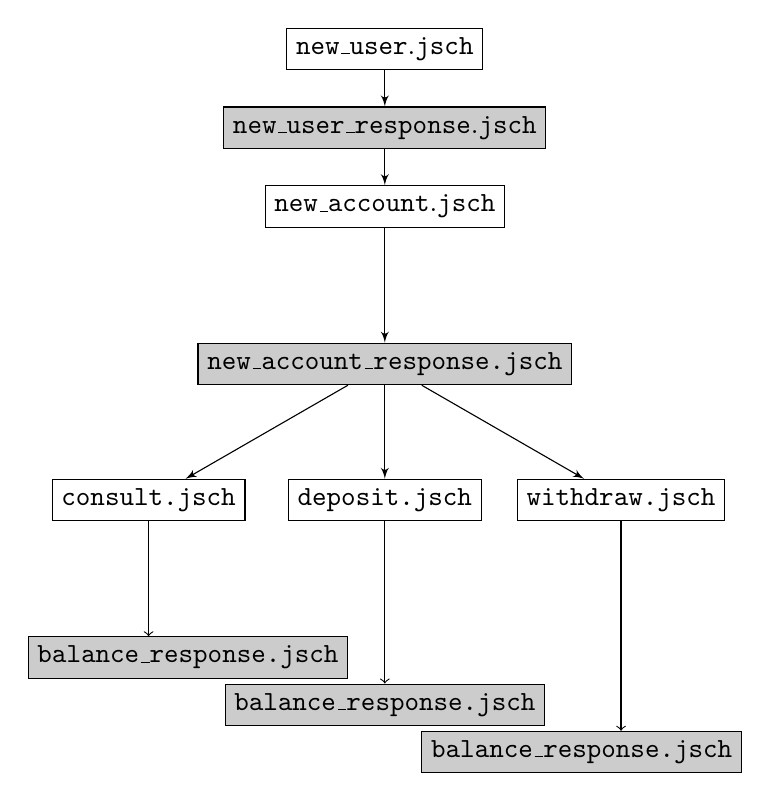
\begin{tikzpicture}
  \tikzset{vertex/.style = {shape=rectangle,draw,minimum size=1.5em}}
  \tikzset{edge/.style = {->,> = latex'}}

  \node[vertex] (new0) at (0,4) {$\mathtt{new\_user.jsch}$};
  \node[vertex, fill=gray!40] (rsp0) at (0,3) {$\mathtt{new\_user\_response.jsch}$};

  \node[vertex] (new) at (0,2) {$\mathtt{new\_account.jsch}$};
  \node[vertex, fill=gray!40] (rsp) at (0,0)
  {$\texttt{new\_account\_response.jsch}$};

  \node[vertex, anchor=south] (consult)  at (-3, -2) {$\texttt{consult.jsch}$};
  \node[vertex, anchor=south] (deposit)  at (0, -2)  {$\texttt{deposit.jsch}$};
  \node[vertex, anchor=south] (withdraw) at (3, -2)  {$\texttt{withdraw.jsch}$};

  \node[vertex, anchor=south, fill=gray!40] (brsp0) at (-2.5,-4){$\texttt{balance\_response.jsch}$};
  \node[vertex, anchor=south, fill=gray!40] (brsp1) at (0,-4.6){$\texttt{balance\_response.jsch}$};
  \node[vertex, anchor=south, fill=gray!40] (brsp2) at (2.5,-5.2){$\texttt{balance\_response.jsch}$};

  \draw[edge] (new0) to (rsp0);
  \draw[edge] (rsp0) to (new);

  \draw[edge] (new) to (rsp);
  \draw[edge] (rsp) to (consult);
  \draw[edge] (rsp) to (deposit);
  \draw[edge] (rsp) to (withdraw);

  \draw[->] (consult.south) to (brsp0.north -| consult);
  \draw[->] (deposit.south) to (brsp1.north -| deposit);
  \draw[->] (withdraw.south) to (brsp2.north -| withdraw);
\end{tikzpicture}
\end{document}